%\begin{figure}[h!]
%    \centering
%    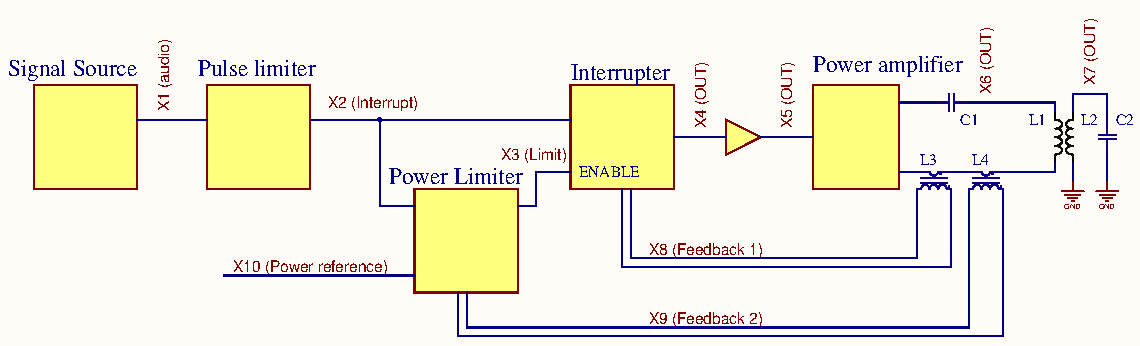
\includegraphics[width=\textwidth]{Skjema/FunksjonsBlokkskjema.pdf}
%    \caption{Block diagram}
%    \label{fig:block}
%\end{figure}

\newpage
\section{Pulse shaper}
\label{sec:pulseshaper}
The purpose of the pulse shaper is to take the input signal $X1$ and transform it to be suitable for a DRSSTC, in addition to not letting harmful signals through. The pulse shaper in this implementation is built separate from the driver. The first step in the pulse shaper is to transform the input signal $X1$ to two level as shown in \cref{fig:schmidt}. Then the triggering signal $X2$ is two level and contains two pieces of information from $X1$, the frequency $f_{X2}$ (tone) and the volume (intensity). \Cref{fig:x2detail} shows the signal X2.

\begin{figure}[H]
\centering
\begin{tikzpicture}[x=16mm,
       every edge/.style = {draw, Straight Barb-Straight Barb},
every edge quotes/.style = {fill=white,font=\footnotesize}
                    ]
%\draw[thick,black, smooth,domain=9:101] plot (\x/10,1);
\draw[thick] (0.5,0) -- (1,0) -- (1,1) -- (2,1) -- (2,0) -- (5,0) -- (5,1) -- (6,1) -- (6,0) -- (7.6,0);
\draw (0,0.5) node {$X2$}; %label

\foreach \x in {1, 2, 5, 6}
    \draw[dashed]  (\x,-0.8) -- ++ (0,1.0);

\draw   (1.0,-0.3) edge ["$T_H$"] ++ (1,0)
        (5.0,-0.3) edge ["$T_H$"] ++ (1,0)
        (1.0,-0.6) edge ["$T_P$"] ++ (4,0);
    \end{tikzpicture}
    \caption{Detail view of signal $X2$}
    \label{fig:x2detail}
\end{figure}{}

Where the frequency $f_{X2}=\frac{1}{T_P}$ is given by the time $T_P$ between the positive flanks of the signal. This is the base harmonic of the acoustic tone heard at the output of the system. The volume is given by the duty cycle of the pulses witch is the relationship between the pulse being high $T_H$ and the total period $T_P$ of the pulse. \Cref{fig:tones} shows different tones,

\begin{figure}[H]
    \centering
    \begin{tikztimingtable}
        X2 & 2L 1H 7L 1H 7L 1H 7L 1H 7L\\
        X2 & 2L 1H 5L 1H 5L 1H 5L 1H 5L 1H 5L 1H 1L\\
    \end{tikztimingtable}
    \caption{Different tones}
    \label{fig:tones}
\end{figure}{}

and \cref{fig:volumes} shows different volumes.

\begin{figure}[H]
    \centering
    \begin{tikztimingtable}
        X2 & 2L 1H 7L 1H 7L 1H 7L 1H 7L\\
        X2 & 2L 3H 5L 3H 5L 3H 5L 3H 5L\\
    \end{tikztimingtable}
    \caption{Different volumes}
    \label{fig:volumes}
\end{figure}{}

We also need to prevent harmful signals, this is done by limiting the duty cycle of the pulses as well as limiting the frequencies allowed. The duty cycle of the pulses is limited by choosing a maximum time $T_H$ the pulse is allowed to be high, this time is independent of the frequency. This means the preset max duty cycle is dependent on the frequency of the pulse.
Limiting the frequencies allowed is done by choosing a minimum time $T_P$ after a pulse goes high until the $X2$ is allowed to go high again.

\section{Interrupter}
\label{sec:interrupter}

The interrupter generates the signal which drives the resonant circuit (coil rig) at its resonant frequency $f_0$. As long as the input signal X2 is high the output produces a square wave with fundamental frequency $f_0$. It does this by the means of a positive feedback loop. The feedback signal X8 is retrieved with a sensing transformer around the output wire from the power amplifier, before being clamped, rectified, and schmidt triggered. This results in a cleaned up normalized representation of X8, lets call this signal X8'. The flanks of X8' represents when the output current passes zero (this is when we want to switch the polarity of the output). X8' is fed to the output via gates controlled by a latch. One of the outputs is inverted (for push-pull operation). This circuit is shown in \cref{fig:interrupter}, U1A is the latch witch is central to the operation of the interrupter. It has Four inputs SD, CP, D, and RD, wich are 'Set Data' (active low), 'Clock Pulse', 'Data', and 'Reset Data' (active low) respectively. And two outputs; Q wich is the normal output, and Q inverted wich is the inverted of Q at all times, Q inverted is unused in this circuit.

\begin{figure}[h!]
    \centering
    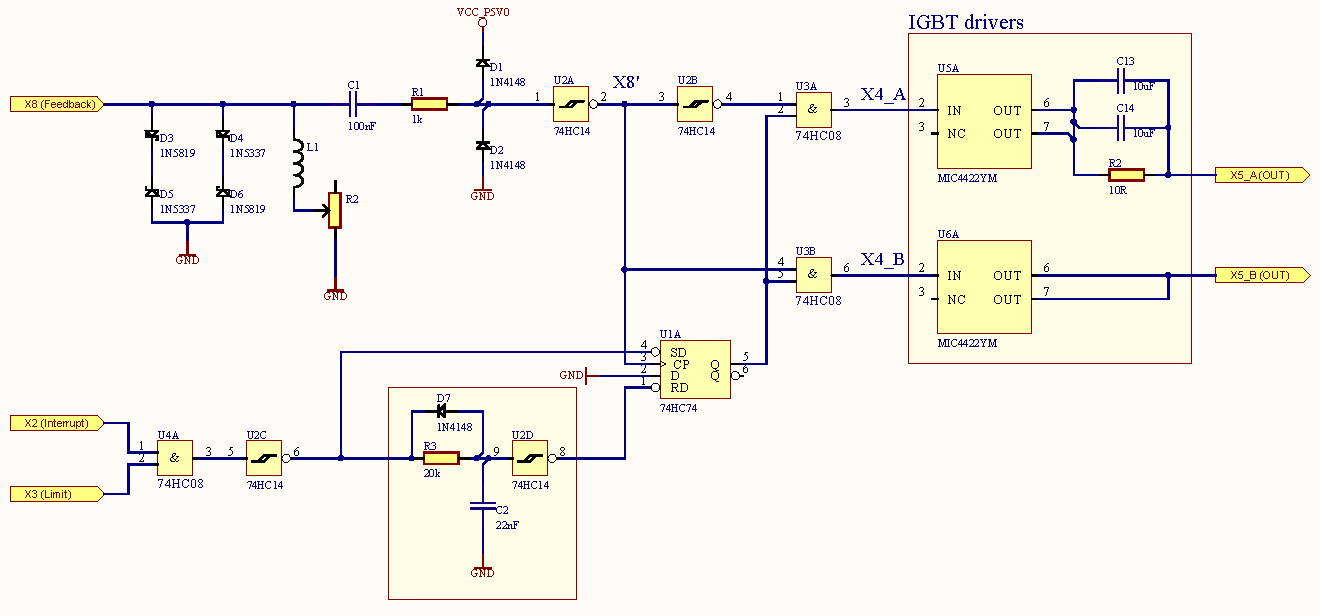
\includegraphics[width=0.9\textheight,angle=-90]{Skjema/TK514_Interrupter.pdf}
    \caption{Interrupter (TK514)}
    \label{fig:interrupter}
\end{figure}

\newpage

Initially no current is flowing in the resonant circuit therefore no voltage is present on X8, but because of C1 the the input of U2A is undefined, let us look at the case of the output of U2A being high and the input X2 being low. Then the initial values of the signals are as shown in \cref{fig:int_timing}, SD is high (inactive) CP is high, D is low, RD is low (active), Q is low, X4\_A and X4\_B is low.

\begin{figure}[!ht]
    \centering
    \begin{tikztimingtable}
        X2      & 2L 19H 0.5H 10.5L\\
        X8'     & 2H 1H 19.5{1C} N(A1) 4{1C} 6H\\
        SD      & 2H 19L 0.5L 10.5H\\
        CP      & 2H 1H 24{1C} 5H\\
        D       & 32L\\
        RD      & 2L 28H 2L\\
        Q       & 2L 1H 19H N(B1) 10L\\
        X4\_A   & 2L 1L 19{1C} 10L\\
        X4\_B   & 2L 1H 19{1C} 10L\\
        \extracode
        \tablerules
        \begin{pgfonlayer}{background}
            \draw [help lines] (A1) -- (B1);
        \end{pgfonlayer}
    \end{tikztimingtable}
    \caption{Timing diagram for interrupter}
    \label{fig:int_timing}
\end{figure}{}

When X2 goes high the Set Data (SD) input of the latch U1A goes low and is activated, Reset Data RD goes high (inactive), and thus the output Q goes high. This enables the and gates U3A and U3B and allows X8' to pass through, X4\_B goes high and X4\_A remains low, this causes a step response in the resonant circuit. The feedback transformer is oriented such that this current direction gives a negative voltage on X8 and thus still low signal on the input of U2A. When the current direction changes the signal on the input of U2A goes from low to high and X4A goes high and X4B goes low. This reverses the voltage on the resonant circuit in phase with the step response and triggers an additional step response in phase with the already ongoing one. This cycle continues until X2 goes low. When X2 goes low SD goes low (inactive), but Q is still high until the next negative flank on X8 (inverted through U2A). When D (wich is strapped low) is clocked through the latch, Q goes low and both X4\_A and X4\_B goes low. And no further energy is supplied to the resonant circuit and the step response completes. In the case of the initial value of the output of U2A being low X4\_A would go high first instead of X4\_B and X8 would go high right away. Prompting X4\_A and X4\_B to invert immediately and switch the output while the current is not zero. Then the rest of the events happen as explained above. \todo{Analysere/Diskutere initialverdi på U2A}

\subsubsection{Phase Lead}
\label{sec:phaselead}
The function of L1 and R2 is to introduce a phase lead on the voltage of X8 in relation of the current on X8. The purpose of this is to compensate for propagation delays in the circuit and for switching delays in the transistors in the power amplifier. As the circuit is inductive, the voltage will lead the current. By adjusting the value of R2 the relation between the inductance and resistance is changed and thus the phase angle is changed. Thus the time between when the voltage crosses zero and the current crosses zero can be adjusted. This time should theoretically be equal to the time it takes the feedback signal X8 to propagate through the logic and for the transistors (IGBTs) in the power amplifier to turn on or off. So that we will switch when the current in the resonant circuit is zero (Zero current switching). This is to reduce energy lost from the resonant circuit and to minimize power burned in the transistors (when switching). From the datasheets we have the propagation delays $t_{pd}$ for the different devices in the propagation path shown in \cref{tab:tpd}. The there are two propagation paths one path contains one schmidt trigger (74HC14) more than the other, also the propagation delay in the mosfet drivers (MIC4422YM) differs for rising and falling outputs. The average propagation delay $\overline{t_{pd}}$ from X8 on the input of U2A to X5 on the output of the mosfet drivers is then given by \cref{eq:tpd} and results in $\overline{t_{pd}} =$ 58 ns typical and 137,5 ns maximum.

\begin{equation} \label{eq:tpd}
    \overline{t_{pd}} = t_{inv} + \frac{t_{inv}}{2} + t_{and} + \frac{t_{driv R}+t_{driv F}}{2}
\end{equation}

In addition the delays from hysteresis in U2A $t_h$ and switching delays in the transistors in the power amplifier $t_{sw}$ should be added to the desired phase lead $t_{d}$. Resulting in the desired phase lead $t_{d}$ being given by \cref{eq:td}.

\begin{equation} \label{eq:td}
    t_d = t_{h} + t_{pd} + t_{sw}
\end{equation}

The feedback signal X8 should have sufficiently high voltage so that delays from hysteresis $t_h$ in U2A is neglible. Delays in the IGBT is read from the datasheet and presented in \cref{tab:tigbt} if we add the delay at 25 $^{\circ}C$ to the nominal $t_d$ and the delay at 150$^{\circ}C$ to the maximum $t_d$, we get a $t_d$ of 141 ns nominal and 258 ns maximum.

Since there are no other resistances in the circuit than R2, as R1 is in series with both a capacitor and the input of the logic gate U2A and can be considered close to infinite in relation to R2, the phase angle is given by \cref{eq:theta}.

\begin{equation} \label{eq:theta}
    \theta = {\tan}^{-1}\frac{X_{L_1}}{R_2} = {\tan}^{-1}\frac{\omega L_1}{R_2} = {\tan}^{-1}\frac{2 \pi f_0 L_1}{R_2}
\end{equation}

And thus the desired phase lead is given by \cref{eq:tdl}, and the relation between $L_1$ and $R_2$ is given by \cref{eq:lr}.

\begin{equation} \label{eq:tdl}
    t_{d} = \frac{\theta}{\omega} = \frac{\theta}{2 \pi f_0}
\end{equation}

\begin{equation} \label{eq:lr}
    \frac{L_1}{R_2} = \frac{\tan(\theta)}{\omega} = \frac{\tan(\omega t_{d})}{\omega} = \frac{\tan(2 \pi f_0 t_{d})}{2 \pi f_0}
\end{equation}

Given a $f_0$ of 110kHz and a desired $t_d$ of 141 ns nominal and 258 ns maximum we get $\frac{L}{R} = 1,4 \cdot 10^{-7}$ s nominal and $\frac{L}{R} = 2,6 \cdot 10^{-7}$ s maximum. The total magnitude $|Z_L|$ of the impedance $Z_{L}$ of $L_1$ and $R_2$ should give a sufficiently high voltage $U_{X8}$ so that the delay due to hysteresis in U2A is negligible, but not too high voltage for the zener diodes D3-D6 to handle. The equation for $|Z_L|$ is shown in \cref{eq:zl}.

\begin{equation} \label{eq:zl}
    |Z_{L}| = \sqrt{{R_2}^2 + (2 \pi f_0 L_1)^2}
\end{equation}

The relation between the peak voltage $|U_{X8}|$ over $R_2$ and $L_1$ is shown in \cref{eq:ux8} assuming X8 is sinusiodal.

\begin{equation} \label{eq:ux8}
    |U_{X8}| = |Z_L| |I_{X6}| \frac{n1}{n2}
\end{equation}



\begin{table}[]
    \centering
    \begin{tabular}{c|c|c|c}
                &   Device              & $t_{pd}$ Typ (ns)   & $t_{pd}$ Max (ns) \\
        $t_{inv}$ &   74HC14              & 12            & 25\\
        $t_{and}$ &   74HC08              & 10            & 20\\
        $t_{driv R}$& MIC4422YM Rising    & 20            & 80\\
        $t_{driv F}$& MIC4422YM Falling   & 40            & 80
    \end{tabular}
    \caption{Propagation delays for devices}
    \label{tab:tpd}
\end{table}

\begin{table}[]
    \centering
    \begin{tabular}{c|c|c}
                            & $T_J = 25 ^{\circ}C$ & $T_J = 150 ^{\circ}C$ \\
        Turn-On Delay Time (ns)  & 46                & 31    \\
        Turn-Off Delay Time (ns) & 120               & 210
    \end{tabular}
    \caption{Turn on and off delays in the IGBT IRG4PC50WPbF}
    \label{tab:tigbt}
\end{table}

\subsubsection{Reset network}
\label{sec:reset_net}
The function of the network connected to the reset (RD) of the latch (U1A) is to reset the latch after a delay in the case that a zero crossing is not detected on X8 after X2 goes low. Note the inverting schmidth triggers U2C and U2D on both sides of the network. When X2 goes high the input of U2D goes low immediately due to the capacitor C2 being discharged through D7, but when X2 goes low the capacitor C2 will be charged through R3 and there will be a delay before the latch is reset. The time constant of R3 C2 is $\tau = 440 \cdot 10^{-6} s$, the positive going threshold voltage of the inverting schmitt trigger (74HC14) is $T^+ = 2,5V$ Wich is half of the supply voltage VCC\_P5V0. We know that a capacitor is charged to $0,5 \cdot$ VCC (where VCC is the applied voltage) after $0,7 \tau$, thus the filter R3 C2 together with U2D introduces a delay of $0,7 \tau = 308\mu s$, or if we have a resonance frequency $f_0$ of 110 kHz a delay of about 3,4 periods $T = \frac{1}{f_0}$.

\subsubsection{Input clamping and protection}
D3-D6 are protection diodes which clamp the feedback signal to safe voltages. The network L1 and R2 introduces a tunable phase lead on the voltage. C1 and R1 is a filter to remove noise. D1 and D2 clamps the voltage to 0-5V.

\subsubsection{IGBT Drivers}
U5A and U6A are transistor drivers wich amplify X4 and step up the voltage from 5V to 18V

%%%%%%% Stikkord
%The output of T1 is loaded with a pair of zener diodes with ultrafast diodes to block the slow recovery of the zeners (they are not allowed to be forward biased).  Since the transformer ratio is ~1:1000, by normal transformer action, the current should be 1/1000th of the primary current, and the voltage should be 1000X greater.

%The square wave is also passed through a capacitor to ensure only AC content is passed

%To further protect the logic gate of U1, we have a pair of fast logic diodes to clamp any voltage excursions to the supply rails.

%There are some tricks used to make the JK flip flop (U2) to operate properly in the circuit.  As shown when the interrupter goes HI, CLR\ is LOW.  This puts Q\ in a HI state.  Now, we see that there is a inverter (part of U1) that feeds from the interrupter signal, with its output feeding into an RC circuit and then another inverter.  What this does is delay the HI input to the PRE on the flip flop.  Note that before the PRE is HI, the output from the flip flop is whatever present on CLR\.  If we did not delay the input to PRE, then our interrupter pulse would never be passed along to the gate driver ENABLE (pin 3 on the UCC3732X).  Also note that the flip flop only does its synchronized shut down when PRE is high.  So this leads to choosing what value we want to use for the RC (R9 and C14).  I typically size it so that t=RC=1.5P, where P is the period (in seconds) for 1 RF cycle at the intended operating frequency.  Example, the DRSSTC-1 operates near 60khz, so 1 cycle is 16.67uS, so I would want an RC of about 25uS (whereas I use 22uS).  The important thing is that PRE does not go LOW before the flip flop does its synchronization.  You must allow for at least 1 full cycle of operation after the interrupter has gone LOW for the flip flop to act.  To be on the safe side, you could size the RC to be 3*P.

\newpage
\section{Limiter}
\label{sec:limiter}

The limiter prevents overcurrent in the coil rig by disabling the interrupter when the peak current rises above a preset level. The limiter is shown in \cref{fig:limiter}

\begin{figure}[h!]
    \centering
    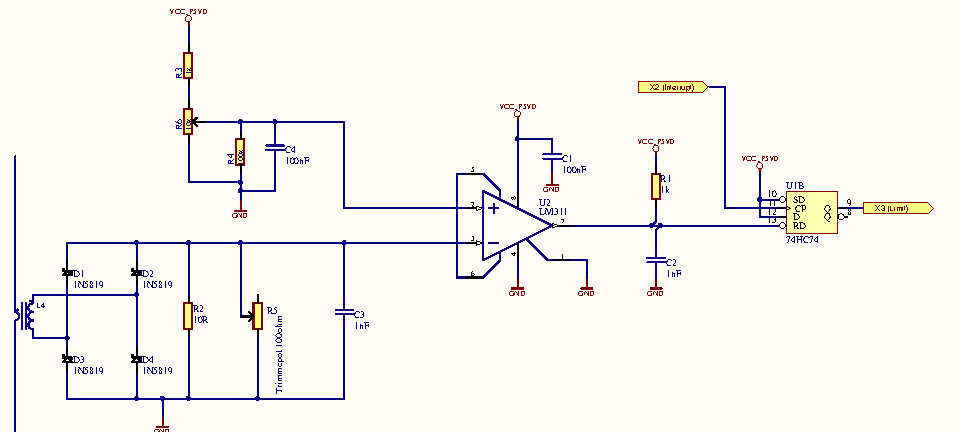
\includegraphics[width=\textwidth]{Skjema/TK513_Limiter.pdf}
    \caption{Limiter}
    \label{fig:limiter}
\end{figure}

The feedback signal is retrieved from the primary resonant circuit via the feedback transformer L4. The diodes D1-D4 is a full bridge rectifier, schottky diodes are used for low propagation delay. The rectifier is loaded with R2 and C3, R2 and C3 also functions as a noise filter with a limit frequency $f_c$ of 16MHz given by \cref{eq:fc}.

\begin{equation} \label{eq:fc}
    f_c = \frac{1}{2 \pi R_2 C_3}
\end{equation}

The rectified signal is fed into a comparator, the other input of the comparator is connected to a variable voltage controlled by a potentiometer. R3 is to set the highest level the variable voltage can be set to. R4 is to pull the input of the comparator low in the case that the potentiometer is disconnected.

The relation between the (peak) current in the primary resonance circuit and the (peak) voltage on the input of the comparator is given by \cref{eq:limittrans}.

\begin{equation} \label{eq:limittrans}
    \frac{U_{X9'}}{I_{X6}} = \frac{n_1}{n_2} \cdot \frac{R_2}{\sqrt{1+(2 \pi 2 f R_2 C_3)^2}}
\end{equation}

\todo{Check equation}

Where $\frac{n_1}{n_2}$ is the winding ratio of the feedback transformer, $I_{X6}$ is the current running in the primary resonance circuit, f is the frequency of $I_{X6}$ (half the frequency of the signal on the input of the comparator because of the full bridge rectifier). Given $n_1 = 1$, $n_2 = 100$, $R_2 = 10\Omega$, $C_3 = 1$nF, f = 110kHz, we get 0,1 Volts per Ampere.

If the voltage of the rectified feedback signal over R2 is higher than the voltage set by the potentiometer the output of the comparator goes low and resets the latch. The data input of the latch is connected to VCC, on the next positive flank of the interrupt signal X2 the data will be clocked to the output and the output will go high.

R5 is to give the possibility to tune the resistance of R2 by removing R2 from the PCB and mounting R5 instead, R5 then replaces R2 in the calculations above.

The output of the latch X3 is connected to the interrupter, as explained in \cref{sec:interrupter}. A low signal stops the output of the interrupter. A high signal allows the interrupt signal X2 to control the output.


\begin{figure}
    \centering
    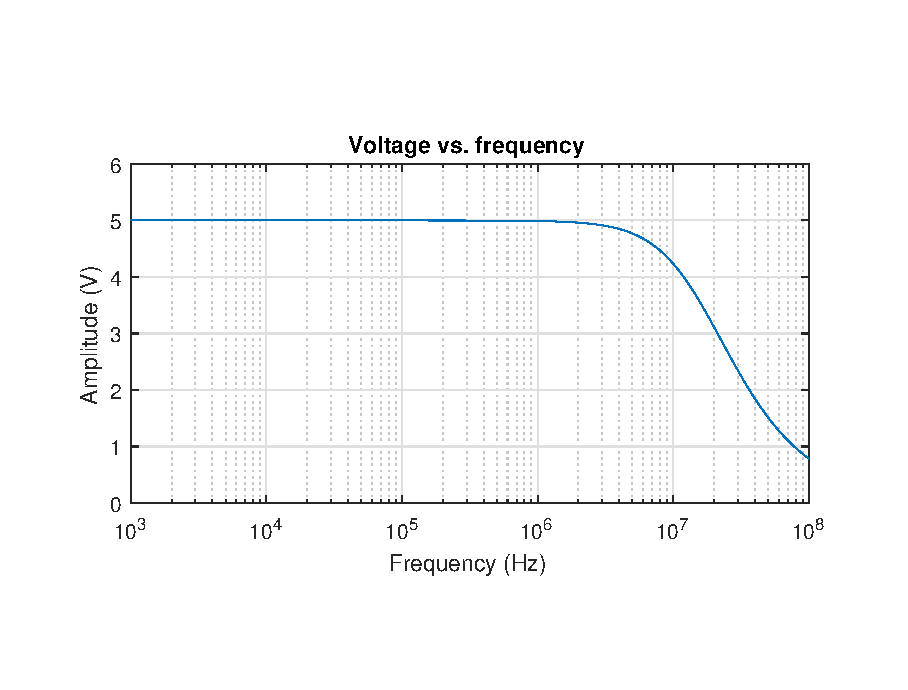
\includegraphics[width=\textwidth]{img/LimiterTransfer.eps}
    \caption{I=50A}
    \label{fig:limitertransfer}
\end{figure}


%%%%%% Stikkord
%The output from the rectifiers is then again loaded down with 100 ohms.  This 100 ohms is to keep the impedance at the comparator (U6) input low, making it somewhat noise immune.  This technique works very well, and without the 100 ohm resistor in place, I find the circuit will falsely trigger on noise.  C15 provides extra noise filtering.


\newpage
\section{Power Amplifier}

The purpose of the power amplifier is to amplify the signal coming from the interrupter X5 and drive the resonant circuit with a high voltage VCC\_HVDC. The power amplifier is shown in \cref{fig:tk531}, note that the feedback transformer L4, as well as the secondary resonant circuit L2 and C2 is not shown for simplicity. The feedback transformer L3 is included in the figure.

\begin{figure}[h!]
    \centering
    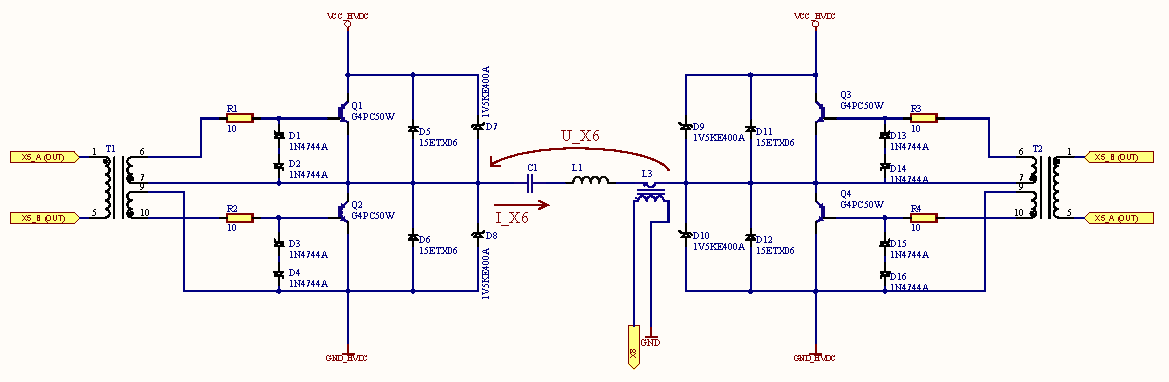
\includegraphics[width=0.9\textheight,angle=-90]{Skjema/TK531_Utgangstrinn_r.pdf}
    \caption{Power Amplifier}
    \label{fig:tk531}
\end{figure}

The power amplifier is a full bridge inverter using Isolated Gate Bipolar Transistors (IGBTs), IGBTs are chosen over MOSFETs due to IGBTs having lower forward voltage drop at higher voltages and currents. The IGBTs are Q1 - Q4.The 1N4744A diodes (15V Zener) is there to clamp the gate voltage to protect the gate of the IGBT from over voltage. The 10 Ohm resistors is to protect from overcurrent. The 1V5KE400A schottky diodes are to protect the IGBTs from reverse voltage transients. The 15ETX06 diodes are there to recycle the leftover energy into the bus capacitors in the power supply when we have stopped switching, as IGBTs does not conduct reverse current. L3 is the current sense feedback transformer, L1 and C1 is the primary resonant circuit. T1 and T2 are gate drive transformers. The supply voltage VCC\_HVDC is 160VDC.

\subsection{Gate drive transformers}
T1 and T2 are gate drive transformers, the purpose of the gate drive transformers is to isolate the low voltages in the interrupter from the higher voltages in the power amplifier, as well as to switch the phase for half of X5 the signal driving the transistors.

%%%%%%% Stikkord
%the anti-parallel diodes in the IGBT recycles the leftover energy into the main bus capacitors as the current rings down.

\newpage
\section{Resonant circuit}
\label{sec:resonant}

The resonant circuits step up the voltage from 160VDC to a voltage high enough to create electric arcs. The resonant circuit consists of two parts the primary resonant circuit; $R_1$, $C_1$, $L1$, and the secondary resonant circuit; $L_2$, $R_2$, $C_2$, $G_1$. The resonant circuit is shown in \cref{fig:spolerigg1}.

\begin{figure}[H]
    \centering
    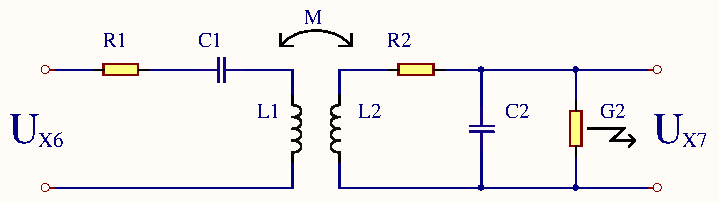
\includegraphics[width=\textwidth]{Skjema/Spolerigg1_r.pdf}
    \caption{Resonant circuit}
    \label{fig:spolerigg1}
\end{figure}

The input signal to the resonant circuit $X6$ is the square wave output from the power amplifier. When the interrupter first applies a voltage to the primary resonant circuit through the power amplifier the circuit responds with its step response, this is sinusoidal and with a frequency equal to the resonant frequency. When the interrupter detects that the current in the primary resonant circuit passes zero the polarity switches, as explained in \cref{sec:interrupter}, and we get a new step response added to the already existing one. This continues for several cycles. This current is inductively coupled into the secondary resonant circuit, and when the voltage reaches a high enough level an electric discharge happens from the top load of the secondary resonant circuit, this drains energy from the secondary circuit, but the electric discharge continues to grow for a couple of cycles. The wave forms of the signals will be explained in \cref{sec:math}.

The values and the physical shapes of the components in the resonant circuit are important to the operation of the tesla coil. The values of the components will be discussed in \cref{sec:math}.

$L_1$ is the primary coil, and will have few turns and large area.

\begin{equation} \label{eq:}
    L_1 = \sqrt{(L_{1V}\cdot \sin (\theta))^2 + (L_{1H}\cdot \cos (\theta))^2}
\end{equation}

\begin{equation} \label{eq:}
    L_{1V} = \frac{R^2 N^2}{9 \bar{r} + 10 h}, L_{1H} = \frac{R^2 N^2}{8 \bar{r} + 11 h}
\end{equation}


\begin{equation} \label{eq:}
    \bar{r} = \frac{A}{2} + \frac{W}{2}
\end{equation}

\begin{equation} \label{eq:}
    \sin (\theta) = \frac{h}{l}, \cos (\theta) = \frac{W}{l}
\end{equation}

\begin{equation} \label{eq:}
    l = \sqrt{W^2 + h^2}
\end{equation}

\begin{equation} \label{eq:}
    W = \frac{B - A}{2}
\end{equation}

% Harold A. Wheeler, "Simple Inductance Formulas for Radio Coils," Proceedings of the I.R.E., October 1928, pp. 1398-1400

$h$ is height of cone, B diameter top of cone, A diameter base of cone, N number of turns, \bar{r} is effective with of coil $l$ is length of coil, $\theta$ is angle of coil, $L_{1V}$ is the vertical component of the inductance, $L_{1H}$ is the horizontal part of the inductance. \citep{wheeler}.

$L_2$ is the secondary coil and will have many turns and small area.

\begin{equation} \label{eq:l2}
    L_2 = \frac{{\mu}_0 N^2 \pi {r}^2}{l}
\end{equation}

Where ${\mu}_0$ is permeability for vacuum, $N$ is the number of turns, and $l$ is the length of the coil. This equation comes from the long solenoid approximation.

$C_1$ is an ordinary capacitor, the type of capacitor should be chosen to withstand the voltages and current required without degrading. And should have as low resistance as possible.

$C_2$ is the place where we want the electric discharge to happen, and thus $C_2$ must withstand the voltages and currents required without degrading. This is achieved by using the self capacitance of a single conductor as opposed to the more common mutual capacitance of two paralell plates. $C_2$ is placed at the top of $L_2$ and is also known as the top load, the top load can be any shape that does not have sharp corners. The most common shapes are spherical or toroidal. The self capacitance of a spherical top load $C_2$ is given by \cref{eq:c2}.

\begin{equation} \label{eq:c2}
    C_2 = 4 \pi {\epsilon}_0 r_{c}
\end{equation}

Where ${\epsilon}_0$ is the permittivity of vacuum, and $r_c$ is the radius of the sphere. This equation is derived from the capacitance of an spherical paralell plate capacitor where the radius of the outer sphere goes toward infinity.

\begin{equation} \label{eq:}
    
\end{equation}

\todo{Mer utfyllende}
%%%%%%%%%%%%% Stikkord
% Løs kobling mellom primær og sekundær for å ikke laste primærkretsen for mye.
% Må tune primær til samme frekvens som sekundær
% Sekundær bestemmer frekvensen.
% Q verdi?

\section{Power supply}
The power supply for the driver is, as for most electronic systems, critical for the quality of operation. This implementation uses three different power supplies for VCC\_P5V0, VCC\_P18V, and VCC\_HVDC. Wich are 5,0V DC, 18V DC, and 160V DC respectively. VCC\_P5V0 supplies the logic circuits, and should supply enough power for this, as well as not introducing noise to the signals in the logic circuits. VCC\_P18V supplies power to the transistor drivers in the interrupter, and has the same requirements as VCC\_P5V0. VCC\_HVDC supplies the power amplifier, and should be able to supply large peak currents with low resistance and delay, as seen from the simulation of the current drawn by the primary resonant circuit in \cref{fig:fblinsim} in \cref{sec:mod_fb}. How this can be achieved is assumed well understood and documented in the field of electronics and will not be discussed any further.

\section{Shielding}
\label{sec:shielding}
The electric discharge produced by a tesla coil generates a large dynamic electromagnetic field\todo{How large?}. This will induce currents in any conductor close to the tesla coil. This must be taken into account when doing pcb layout and designing the chassis for the tesla coil driver. How this can be achieved is assumed well understood and documented in the field of electronics and electrodynamics and will not be discussed any further.

\section{Optical channel}
\label{sec:optical}

As mentioned in \cref{sec:shielding} there is electromagnetic noise present when the tesla coil is used and a robust channel is needed for signal $X2$ because this signal is transmitted from the pulse shaper to the tesla coil driver, wich as mentioned in \cref{sec:pulseshaper} are physically located in different chassis some distance apart. For this plastic optical fibre is chosen. To further increase the robustness the signal $X2$ is modulated. The robustness and possible noise introduced in this channel is not discussed further as it can be treated as an isolated problem and is assumed well understood and documented in the field of electronics. A diagram of the optical channel is shown in \cref{fig:opticalchannel}.

\begin{figure}[H]
    \centering
    \tikzstyle{int}=[draw, fill=yellow!20, minimum size=2em]
    \tikzstyle{init} = [pin edge={to-,thin,black}]
    \begin{tikzpicture}[node distance=2.5cm,auto,>=latex']
        \node [int, pin={[init]above:$CW$}] (a) {tx};
        \node (b) [left of=a,node distance=2cm, coordinate] {a};
        \node [int] (c) [right of=a] {rx};
        \node [int] (d) [left of=a] {Pulse shaper};
        \node [int] (e) [right of=c] {Interrupter};
        \node [coordinate] (end) [right of=c, node distance=2cm]{};
        \path[->] (d) edge node {$X2$} (a);
        \path[->] (a) edge node {$PWM$} (c);
        \draw[->] (c) edge node {$X2$} (e) ;
    \end{tikzpicture}
    \caption{Diagram of optical channel}
    \label{fig:opticalchannel}
\end{figure}

Where $CW$ is the carrier wave used to modulate the signal $X2$, $PWM$ is the modulated signal $X2$. The blocks tx and rx are the optical transmitter and reciever.